\chapter{Обзор проектов по созданию инструментов инженерии знаний}\label{ch:ex-solutions}
Рассмотрим современные системы и средства, осуществляющие преобразования текстовых описаний и объектных моделей, а также универсальные средства обратной инженерии, по текстам восстанавливающие графические модели. При обзоре того или иного средства обратим внимание на то, согласуются ли используемые им нотации с существующими стандартами, и есть ли возможность передачи и использования входных и выходных моделей и описаний современными инструментальными средствами.

%При обзоре того или иного средства обратим внимание на то, какие преобразование описывает средство, согласуются ли используемые им нотации с существующими стандартами, и есть ли возможность передачи и использования входных или выходных артефактов системы другими программными инструментами или системами.

\section{Интегрированная среда для моделирования предметных областей (itSIMPLE)}

    \begin{figure}[h]
        \center{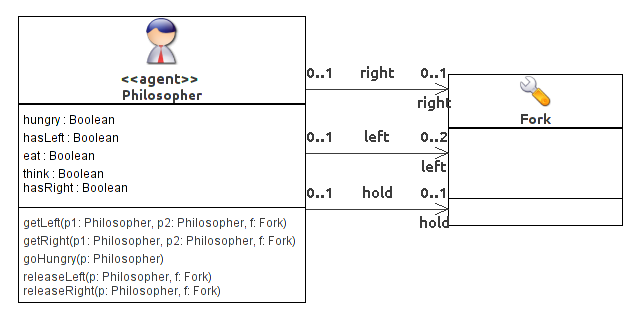
\includegraphics[width=0.8\linewidth]{its-domain}}
        \caption{Диаграмма классов предметной области в itSIMPLE}
        \label{img:its-domain}

    \end{figure}
    
    \begin{figure}[h] 
        \center{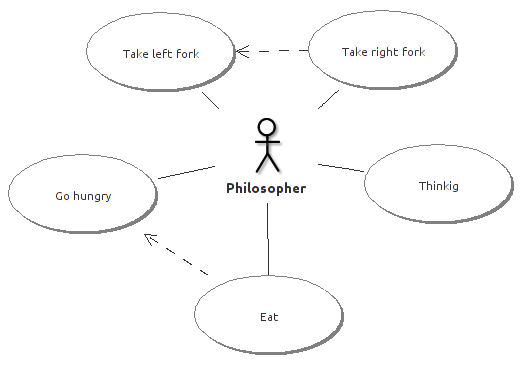
\includegraphics[width=0.8\linewidth]{its-use-case}}
        \caption{Диаграмма вариантов использования в itSIMPLE}
        \label{img:its-use-case}
    \end{figure}

    \begin{figure}[h] 
        \center{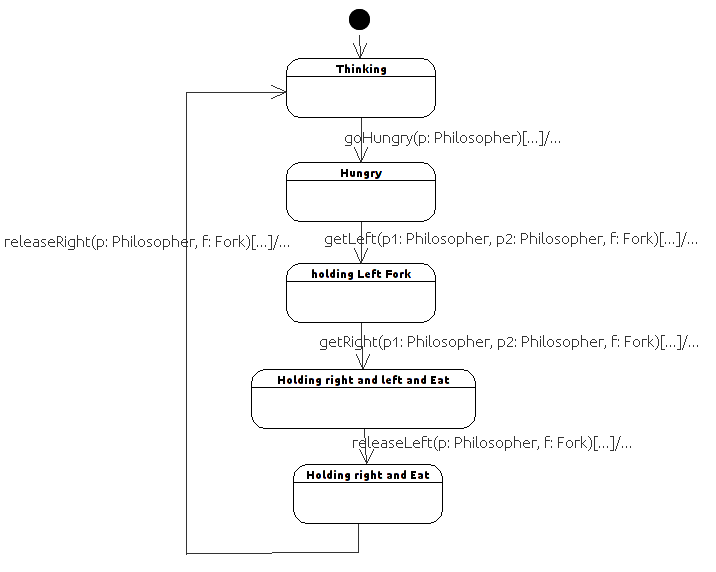
\includegraphics[width=0.9\linewidth]{its-states}}
        \caption{Диаграмма состояний объектов в itSIMPLE}
        \label{img:its-states}
    \end{figure}

    

    Одной из сред поддержки процессов, связанных с планированием, является среда itSIMPLE \cite{itsimple} (Integrated Tools Software Interface for Modeling PLanning Environments).
 В ней предложено использовать UML-модели для описания знаний систем планирования. Описанные модели можно автоматически транслировать на PDDL, а затем подать на вход планировщикам.
 Полученный план затем можно визуализировать внутри среды.
 Под визуализацией понимается отображение в виде диаграмм объектов последовательных состояний, через которые проходит система.
 %Так или иначе, средство решает обратную задачу, а не задачу, поставленную в данной работе.

Посмотрим подробнее, какое предложено отображение в данном инструменте. Для описания предметной области используется диаграмма классов, на ней могут присутствовать классы, ассоциации, отношения тип-подтип, а также перечислимые типы. Классы, экземпляры которых могут совершать действия, помечены стереотипом \stype{Agent}.
На рис.~\ref{img:its-domain} показано описание классов предметной области ``Обедающие философы''. Классы могут иметь атрибуты, типом атрибута может быть один из простых типов (\texttt{Boolean}, \texttt{Integer}, \texttt{Float}), а также один из классов, описанных на диаграмме классов. Кроме того, классы содержат в себе описания действий, для которых указываются все параметры, причем первый из параметров не опускается (и не считается за self), как принято в UML. 

Для наглядного описания действий служат диаграммы вариантов использования и диаграммы состояний. Причем, диаграммы вариантов и использования могут использоваться только для дескриптивных целей, т.е.  они не используются в дальнейшем никакими компонентами, из них не извлекается никакой информации для кодогенерации, анализа и т.п. На диаграммах вариантов использования указываются, какие действующие лица существуют в предметной области, какие действия они могут совершать (инициировать), и различные зависимости действий между собой (рис.~\ref{img:its-use-case}).

%На диаграммах состояний моделируется изменение состояний объектов при выполнении действий: в каких состояниях может находиться объект и как осуществляются переходы между состояниями.
%В качестве триггеров на переходах указываются методы с параметрами (\texttt{Action Association}), охранные условия переходов фактически являются частью предусловий, на переходах так же указаны действия, являющиеся частью эффекта, совершаемые при срабатывании перехода, У состояний задаются внутренние условия (\texttt{Internal Condition}) на языке OCL. Часть информации содержится в состояниях объекта, изменяемого действием.
Действия из предметной области авторы itSIMPLE предлагают моделировать при помощи диаграмм состояний. На этих диаграммах действия указываются в роли триггеров на переходах между  состояниями. Предусловия действий авторы предлагают помещать на диаграмму как сторожевые условия на переходах, а эффекты действий~-- как действия на переходах. При этом и предусловия и эффекты описываются как логические выражения на языке OCL
На рис.~\ref{img:its-states} показана диаграмма состояний объекта \texttt{Philosopher}.
Например, для перехода \texttt{releaseRight} указано следующее предусловие:

\begin{alltt}
    p.hold->includes(f) and
    p.right = f and
    p.hasRight = true
\end{alltt}

\noindent и эффект:

\begin{alltt}
    p.think = true and
    p.hold = p.hold->excluding(f) and
    p.hasRight = false
\end{alltt}
%    \begin{figure}[h] 
%        \center{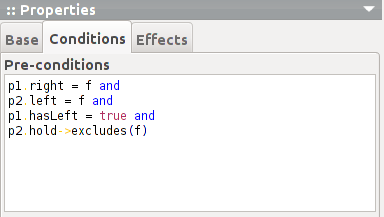
\includegraphics[width=0.5\linewidth]{its_phil_precond}}
%        \caption{Пример описания действия \texttt{getRight} в itSIMPLE}
%        \label{img:its_phil_precond}
%    \end{figure\}                                                                                                          

\begin{figure}[h] 
    \center{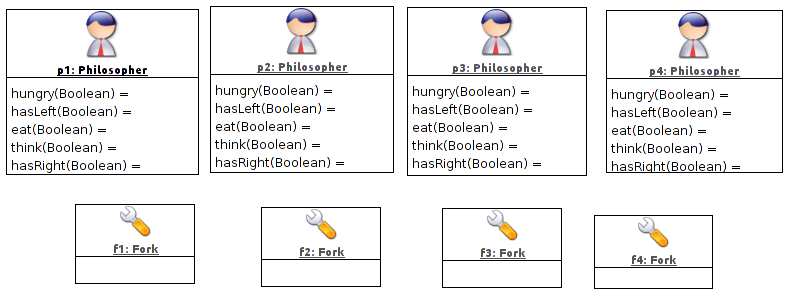
\includegraphics[width=0.8\linewidth]{its-repo}}
    \caption{Диаграмма объектов в itSIMPLE, репозиторий}
    \label{img:its-repo}
\end{figure}

\begin{figure}[h] 
    \center{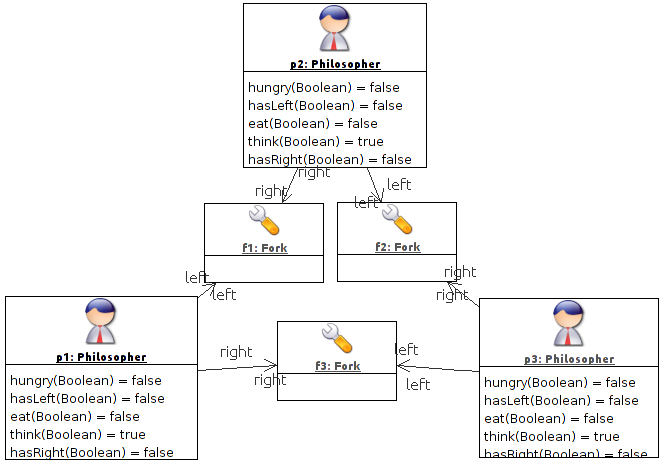
\includegraphics[width=0.8\linewidth]{its-init}}
    \caption{Начальное состояние в виде диаграммы объектов в itSIMPLE}
    \label{img:its-init}
\end{figure}

\begin{figure}[h]
    \centering 
    \begin{minipage}{0.8\linewidth}
        \centering
        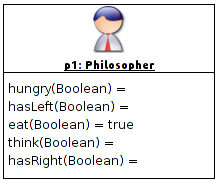
\includegraphics[width=0.35\linewidth]{its-goal}
        \caption{Ограничения на конечное состояние в виде диаграммы объектов в itSIMPLE}
        \label{img:its-goal}
    \end{minipage}
\end{figure}

%Когда генерируется предусловие~--- объединяются свойства исходных состояний для всех объектов, затрагиваемых действием, и дополнительные ограничения, заданные в самих действиях или на диаграмме классов. Эффект действия получается как объединение внутренних условий целевых состояний объектов, которые изменяются в результате совершения действия, а также постусловий операции, которая соответствует описываемому действию. 

Если присмотреться внимательно, становятся видны расхождения между стандартной семантикой элементов UML теми смыслами, которыми те же самые элементы наделяются в itSIMPLE, когда осуществляется преобразования моделей в описания на PDDL. Так сторожевое условие на переходе диаграммы состояний имеет другой смысл, отличающийся от предусловия. Сторожевое условие может быть не выполнено при наступлении триггера и при этом система ведёт себя корректно, в то время как невыполнение предусловия при выполнении действия указывает на внештатную ситуацию (ошибку в найденном плане). В стандарте UML есть вид диаграмм~-- протокольные диаграммы состояний (см.\cite{arlou}),~-- более подходящий для описания действий. На этих диаграммах у переходов отсутствуют сторожевые условия и действия, зато есть пред- и постусловия. Переходы протокольной диаграммы описывают не возможные реакции системы на события, а обязательные смены состояний, не допускающие нарушения условий. 

Следует еще обратить внимание на выражение-эффект, написанное выше. В эффекте полагается, что в правой части относительно знака ``='' выражения принимают значения в момент после завершения действия, а в левой части~--- в момент до начала выполнения действия. Но в стандартной семантике языка OCL это является логическим выражением, а не оператором присваивания. Следуя стандарту OCL, а данном случае для таких целей должен использоваться постфикс \texttt{@pre}, означающий, что значение атрибута берется в момент до совершения перехода.

Для описания условий задач используется три диаграммы объектов: репозиторий объектов задачи (рис.~\ref{img:its-repo}), начальное состояние (рис.~\ref{img:its-init}) и конечное состояние (рис.~\ref{img:its-goal}). В репозитории помещаются все объекты, которые присутствуют в данной конкретной задаче, никаких связей и атрибутов больше на этой диаграмме нет. В диаграмме начального состояния указываются объекты, атрибуты и связи в начальный момент времени. При этом подразумевается, что если связь не указана явно, то она отсутствует. На диаграмме конечного состояния также указываются объекты, атрибуты и связи между объектами, которые хотелось бы видеть в конечном состоянии, то есть, в этом контексте предполагается, что вся не указанная информация об объектах и связях не имеет значения, может как присутствовать в конечном состоянии, так и отсутствовать.
\\

%Семантика, которой наделяются связанные по одинаковым триггерам методы диаграммы состояний,~-- не соответствует стандартной семантике диаграмм конечных автоматов~-- чтобы придерживаться стандарта, для описания действий следовало бы использовать протокольные диаграммы состояний (описаны в~\cite{arlou}).  

%Кроме того itSIMPLE не поддерживает обмен UML-моделями с другими средствами, вся информация сохраняется во внутреннем представлении. Это делает невозможным использование в itSIMPLE моделей, созданных в других средствах, работающих с UML, и наоборот~-- модели, созданные в itSIMPLE, нельзя редактировать с помощью других инструментов и нельзя подавать на вход другим средствам, предоставляющим возможности валидации, трансформации, трансляции моделей на другие языки. Но даже если бы модели были переносимы, то из-за отличной от стандартной семантики, которой наделяет itSIMPLE элементы модели, было бы невозможно для работы с моделью использовать другие инструменты, так как они основываются на стандартной семантике.
Можно сделать вывод, что создателями itSIMPLE применена собственная нотация, внешне сходная с UML, но отличающаяся по семантике. Из-за этого затруднено использование моделей itSIMPLE в UML-средах, поддерживающих стандарт. Попытка запуска исполнения такой модели в UML-среде, не учитывающей особенности itSIMPLE, приведёт к неожиданным результатам. Отход от стандартной UML-нотации частично обесценивает работу инженера знаний, поскольку выполненные им модели, хоть и выглядят похожими на UML-модели, но по сути таковыми не являются.

\section{Графический интерфейс для планирования с объектами (GIPO)}

\begin{figure}[h] 
    \center{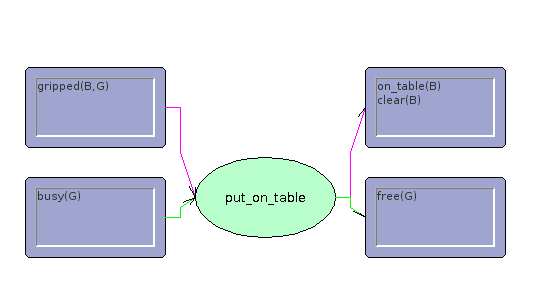
\includegraphics[width=0.8\linewidth]{gipo-transition}}
    \caption{Пример описания действия в среде GIPO}
    \label{img:gipo-transition}
\end{figure}

В 2005 году создавалась GIPO~--- экспериментальная исследовательская среда для инженерии знаний о предметных областях и задачах планирования \cite{gipo}, использовавшаяся в основном для целей обучения.
Основным элементом GIPO является внутреннее представление предметных областей, центром которого являются объекты.
С этим представлением работают остальные элементы инструмента: редакторы, чекеры, валидаторы, внутренние планировщики, аниматоры и т.д. 
Среди возможностей инструмента можно так же назвать поддержку классического планирования, HTN (иерархические  сети задач) планирования, поддержку длительных действий, возможности статического анализа и динамического тестирования плана.

Для того, чтобы GIPO можно было использовать как общее средство моделирования, был реализован транслятор из внутреннего представления $OCL_h$\footnote{$OCL_h$~--- Object Centered Language} в PDDL. 

Типы объектов предметной области (\texttt{sorts}) и предикаты в GIPO соответствуют обычным понятиям PDDL. На их основе определяется понятие состояния для типизированного набора входных переменных. 
Состояние~--- это неименованное множество экземпляров предикатов от каких-либо входных переменных вместе с множеством экземпляров встроенных ограничений (\texttt{ne}, \texttt{eq}, ...). 
В терминах состояний определяются действия, как показано на примере действия \texttt{put\_on\_table} предметной области ``Мир кубиков'' (рис.~\ref{img:gipo-transition}): состояния с исходящими стрелками задают предусловие действия, а с входящими~-- постусловия, в овале находится сам символ действия. 
В терминах экземпляров состояний (подстановки объектов) описываются условия задач.

К сожалению, GIPO использует графические нотации только для описания действий, и эти нотации разработаны конкретно для этого инструмента, не распространены вне его и не имеют соответствия в UML.
Следовательно, не может идти и речи о совместимости модели GIPO с UML инструментами.

Ныне проект не развивается.


\section{Инструмент обратной инженерии MoDisco (Model Discovery)}

Инструмент представляет собой реализацию концепции MDRE \footnote{MDRE~--- Model Driven Reverse Engineering}~--- обратной инженерии, управляемой моделями \cite{modisco}. 

На  рис. \ref{img:modisco_overview} показан общий вид работы средства.
    
    \begin{figure}[h]
        \center{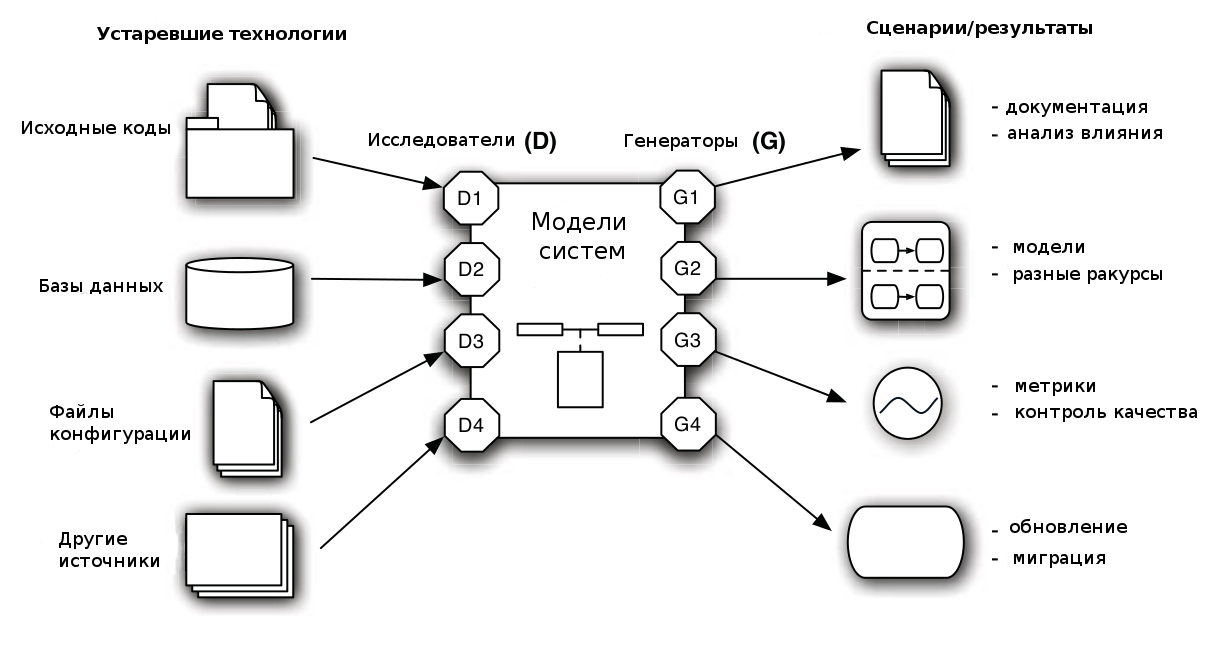
\includegraphics[width=1\linewidth]{modisco_overview2}}
        \caption{Схема работы средства MoDisco}
        \label{img:modisco_overview}

    \end{figure}   

Инструмент позволяет создавать модели различных систем, используя так называемые ``исследователи'' (Discoverers).
В качестве исследуемой системы может выступать и реальная работающая система, например, файловая система одной конкретно взятой машины, или целая сеть машин, и тогда её модель может наглядно показать нам её конфигурацию.

Каждая реальная система описывается метамоделью этой системы, которая описывает устройство целого класса систем (т.е. модель системы~--- это экземпляр её метамодели).
Для того, чтобы MoDisco могло работать с конкретным классом систем, должен быть реализован соответствующий ``исследователь'' и метамодель системы.

После обработки системы ``исследователем'', которая, вообще говоря, может проводиться неоднократно с целью уточнения системы или получения другого представления (viewpoint) системы, получаются модели системы.
Эти модели впоследствии приводятся в соответствие с KDM\footnote{KDM~--- Knowledge Discovery Metamodel}, которая является ядром MoDisco.
В дальнейшем с этими моделями могут проводиться различные действия: они могут быть изменены, пересмотрены, улучшены и т.д.
В конечном счете к моделям могут быть применены M2M/M2T трансформации для получения новых артефактов, изменения существующей системы, создания другого представления системы и т.п.


На данный момент ``исследователи'' существуют в основном только для Java-кода, JAR-архивов, некоторых реляционных баз данных, т.е. для предметных областей и задач планирования (в  т.ч. PDDL) они отсутствуют. 
Кроме того, MoDisco находится в стадии ранней разработки, по нему мало документации и в большинстве своем она не очень понятна.
  

\section{Среда объектно-ориентированной инженерии знаний систем планирования}\label{sec:seminar}   

Данный проект развивается в рамках кафедры системного программирования факультета ВМК. Проект направлен на создание среды объектно-ориентированной инженерии знаний систем планирования. 

По этому проекту в статье \cite{mal-manz} предлагается использовать стандартную нотацию UML и язык объектных ограничений OCL для описания предметных областей и задач планирования. В рамках статьи было предложено задавать описания предметных областей в виде диаграмм классов UML, а пред- и пост-условия~--- в виде ограничений на OCL, начальные условия~--- в виде диаграмм объектов, а цели~--- в виде выражений языка OCL. Предложенная нотация соответствует стандартам.
 
Также, был предложен способ перевода такой нотации в PDDL-описания для планировщика.
А сам генератор был реализован на основе программного средства Acceleo, реализующего стандарт MOFM2T\cite{mofm2t}. Средство Acceleo может работать с любыми моделями, для которых есть реализация метамодели посредством MOF. Такая реализация метамодели UML$^{2.x}$ существует, следовательно, входные данные для реализованного генератора могут создаваться и использоваться в различных UML-редакторах и других средствах, работающих с той же метамоделью.

Задача, которая анализируется и решается в данной дипломной работе, фактически является одной из подзадач данного проекта. Поэтому в работе  предполагается решать эту задачу следуя стандартам и используя стандартные семантики. Кроме того, возможно использование и дополнение общих артефактов проекта, например, UML-профиля области планирования.

\section{Библиотека поддержки планировщиков на языке Java (PDDL4J)}

\begin{figure}[h!]
    \center{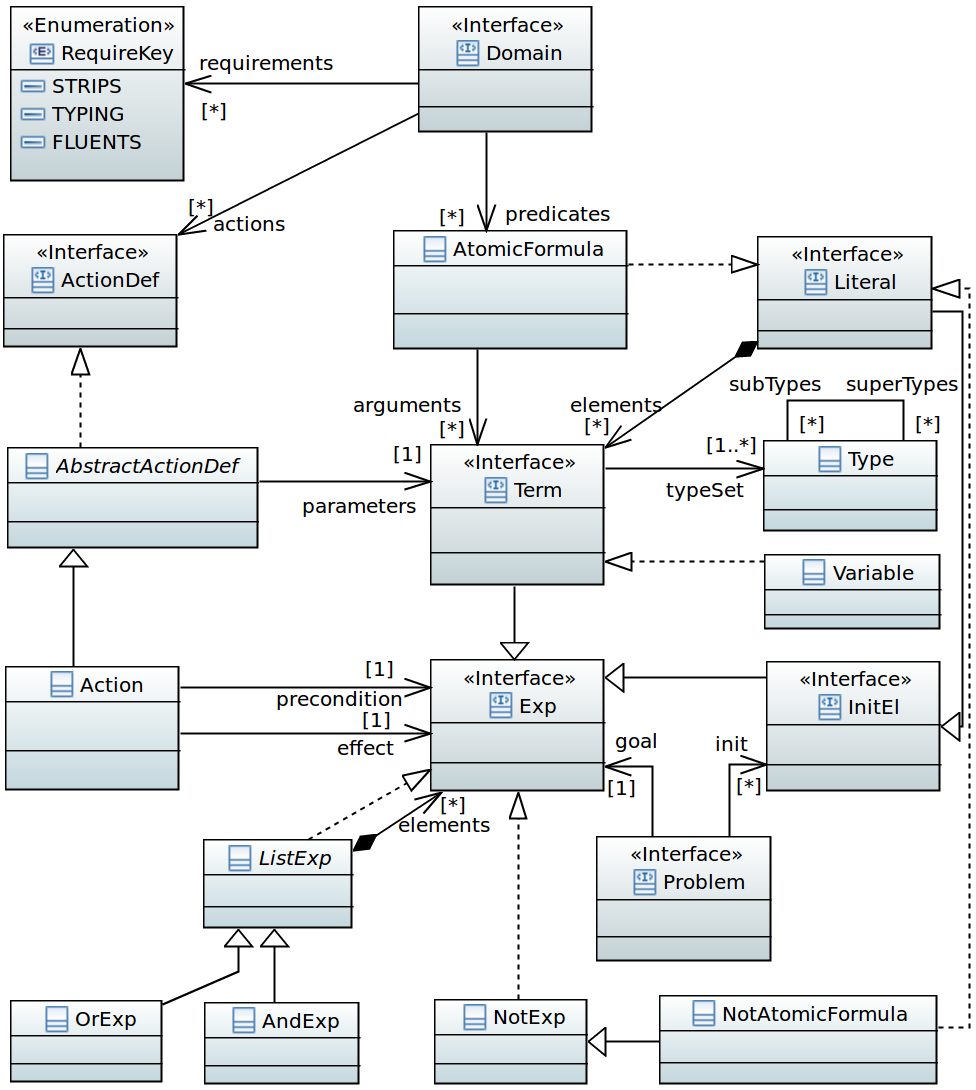
\includegraphics[width=1\linewidth]{pddl4j}}
    \caption{Диаграмма основных компонентов библиотеки PDDL4J}
    \label{img:pddl4j}

\end{figure}   

PDDL4J~--- проект, который создавался для того, чтобы стимулировать развитие планировщиков для PDDL, реализованных на Java\cite{pddl4j}. Библиотека основана на ANTLR\cite{antlr} и может разбирать текстовые PDDL-описания предметных областей и задач планирования. 

Хотя этот проект и не занимается созданием объектных моделей, он интересен тем, что по PDDL-описаниям предметных областей и задач планирования создает в памяти некоторую совокупность объектов и связей между ними представленную библиотечными классами. Эти классы и связи между ними можно рассматривать как своеобразный взгляд на знания систем планирования. 

На рисунке~\ref{img:pddl4j} приведена упрощенная диаграмма классов основных понятий области планирования, которая используется в PDDL4J.
Там тоже есть такие понятия, как предметная область (\texttt{Domain}), которая определяется набором требований, предикатов и действий. С каждым предикатом (\texttt{AtomicFormula}) связан список аргументов, каждый из которых является термом (\texttt{Term}). С каждым действием (\texttt{Action}) связаны параметры действия, предусловие и эффект, представленные выражениями (\texttt{Exp}). В свою очередь термы сами по себе являются выражениями и имеют тип (или несколько типов). Для каждого типа (\texttt{Type}) определены наборы его супертипов и подтипов, так моделируется типизация PDDL. Задачи планирования (\texttt{Problem}) определяются начальным состоянием и целью. Цель задана как некое выражение, а начальное состояние~--- как набор элементов инициализации.

%%%%%%%%%%%%%%%%%%%%%%%%%%%%%%%%%%%%%%%%%%%
\section{Выводы}

%Подавляющее большинство инструментов, реализующих преобразование каких-либо текстовых данных в UML-модели, существует для работы с языками программирования, как правило, объектно-ориентированными, а не с языками представления знаний. Поэтому, использование этих инструментов для решения поставленной задачи невозможно.

Можно видеть, что ни один из рассмотренных инструментов не позволяет преобразовывать входные описания планировщиков в объектные спецификации, представленные UML-моделями. 

В обзоре itSIMPLE мы увидели, что общепринятые элементы UML наделяются новой семантикой. Это неизбежно влечет за собой сужение области применимых к UML-моделям itSIMPLE инструментов. Поэтому стандарты нужно стараться соблюдать.

На примере GIPO мы увидели, что использование собственной нотации чревато тем, что инструмент будет мало востребован, инженеры знаний просто не захотят его использовать, и проект будет заброшен. 

В MoDisco не реализован ``исследователь'' для PDDL, а задача его разработки сопоставима по сложности с задачей разработки такого генератора с нуля.

Разработчики библиотеки PDDL4J не ставили своей целью создание инструмента генерации UML-моделей по PDDL-описаниям, но её можно достроить до такого генератора, реализовав преобразование  промежуточного объектного представления, предоставляемого библиотекой, в UML-модели.

\newpage